\subsection{Question 1}
    \textbf{Give the intermediate representation in TAC for the following expression:}

    \input{TP6/q1}

    \input{TP6/1}

\subsection{Question 2}
    \textbf{For each of the following C functions, give the control flow graph (CFG), the minimized SSA form, and the non-SSA form without parameterized labels (the form that can be used to generate assembly code)}

    \input{TP6/q2}
    \begin{figure}[H]%
                \centering
                \subfloat[\centering]{{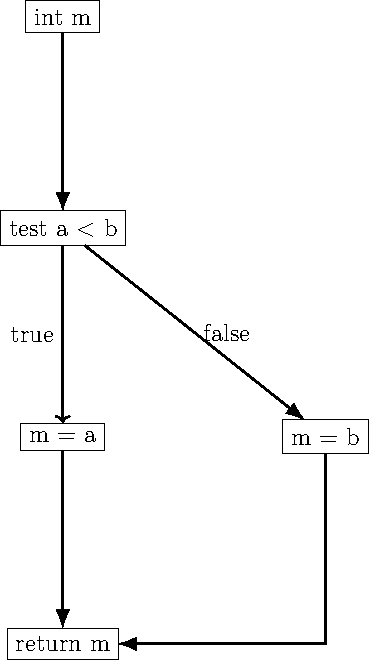
\includegraphics[width=5cm]{img/TP6/cfg_min.pdf} }}%
                \qquad
                \subfloat[\centering ]{{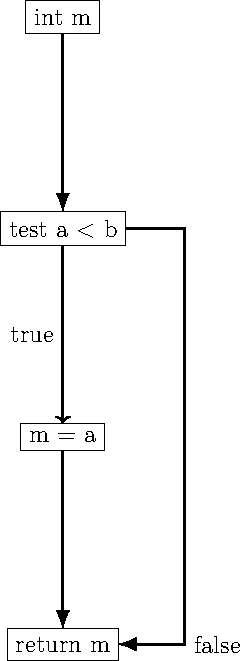
\includegraphics[width=5cm]{img/TP6/cfg_min_alternative.pdf} }}%
                \caption{CFG for min and minAlternative $(a|b|bc)^{*}a$}%
                \label{fig:example}%
            \end{figure}
    \addimg{img/TP6/cfg_squareSum.pdf}{scale=0.5}{CFG for squareSum}{}
    
    Minimized SSA for min:
    \begin{lstlisting}[language = Java , frame = trBL , firstnumber = last , escapeinside={(*@}{@*)}]
min(a0,b0):
    if a0 < b0 then goto body else goto elsebody
body:
    m0 = a0
    goto done(m0)
elsebody:
    m1 = b0
    goto done(m1)
done(m2):
    return m2
\end{lstlisting}
    Minimized SSA for minAlternative:
    \begin{lstlisting}[language = Java , frame = trBL , firstnumber = last , escapeinside={(*@}{@*)}]
minAlternative(a0,b0):
    m0 = b0
    if a0 < b0 then goto body else goto done(m0)
body:
    m1 = a0
    goto done(m1)
done(m3):
    return m3
\end{lstlisting}
    Non minimized SSA for squareSum:
    \input{TP6/square_sum_nm_ssa}
    Minimized SSA
    \input{TP6/square_sum_min_ssa}
    Non minimized non-SSA
    \input{TP6/square_sum_non_ssa}
    Minimized non-SSA
    \input{TP6/square_sum_min_non_ssa}

\subsection{Question 3}
    \textbf{Design a simple algorithm that verifies that a function has no missing return statement. The algorithm should also work for complex functions that contain many if-statements, loops, etc.}

    \input{TP5/3}

